\documentclass[a4paper, amsfonts, amssymb, amsmath, reprint, showkeys, nofootinbib, twoside]{revtex4-1}
\usepackage[english]{babel}
\usepackage[utf8]{inputenc}
\usepackage[colorinlistoftodos, color=green!40, prependcaption]{todonotes}
\usepackage[pdftex, pdftitle={Article}, pdfauthor={Author}]{hyperref}
\usepackage{amsthm}
\usepackage{mathtools}
\usepackage{physics}
\usepackage{xcolor}
\usepackage{caption}
\usepackage{hyperref}
%\hypersetup{colorlinks=true, linkcolor=blue, urlcolor = blue}
\usepackage{amsmath}
\usepackage{amssymb}
\usepackage{graphicx}
\graphicspath{Images}
\usepackage[left=23mm,right=13mm,top=35mm,columnsep=15pt]{geometry} 
\usepackage{adjustbox}
\usepackage{placeins}
\usepackage[T1]{fontenc}
\usepackage{float}
%\usepackage{longtable}
\usepackage{csquotes}
\usepackage{refstyle}
\usepackage{lipsum}

\begin{document}

\title{Emission spectra of Copper, Brass and Iodine using constant deviation spectrometer}
\author{Swaroop Ramakant Avarsekar}
\email{swaroop.avarsekar@niser.ac.in}
\affiliation{School of Physical Sciences, National Institute of Science Education and Research, HBNI, Jatni -752050, India}
\date{\today}

	
\begin{abstract}

\end{abstract}
	
\maketitle

\section{Introduction and Theory}
Constant deviation prism consist of two $30^{\circ}$ prism (PQR and QTS) along with reflecting prism (PRS). The incident ray (AB) on PQ, under certain angle undergoes deviation of 90$^\circ$. 

\begin{figure}[H] %  figure placement: here, top, bottom, or page
	\centering
	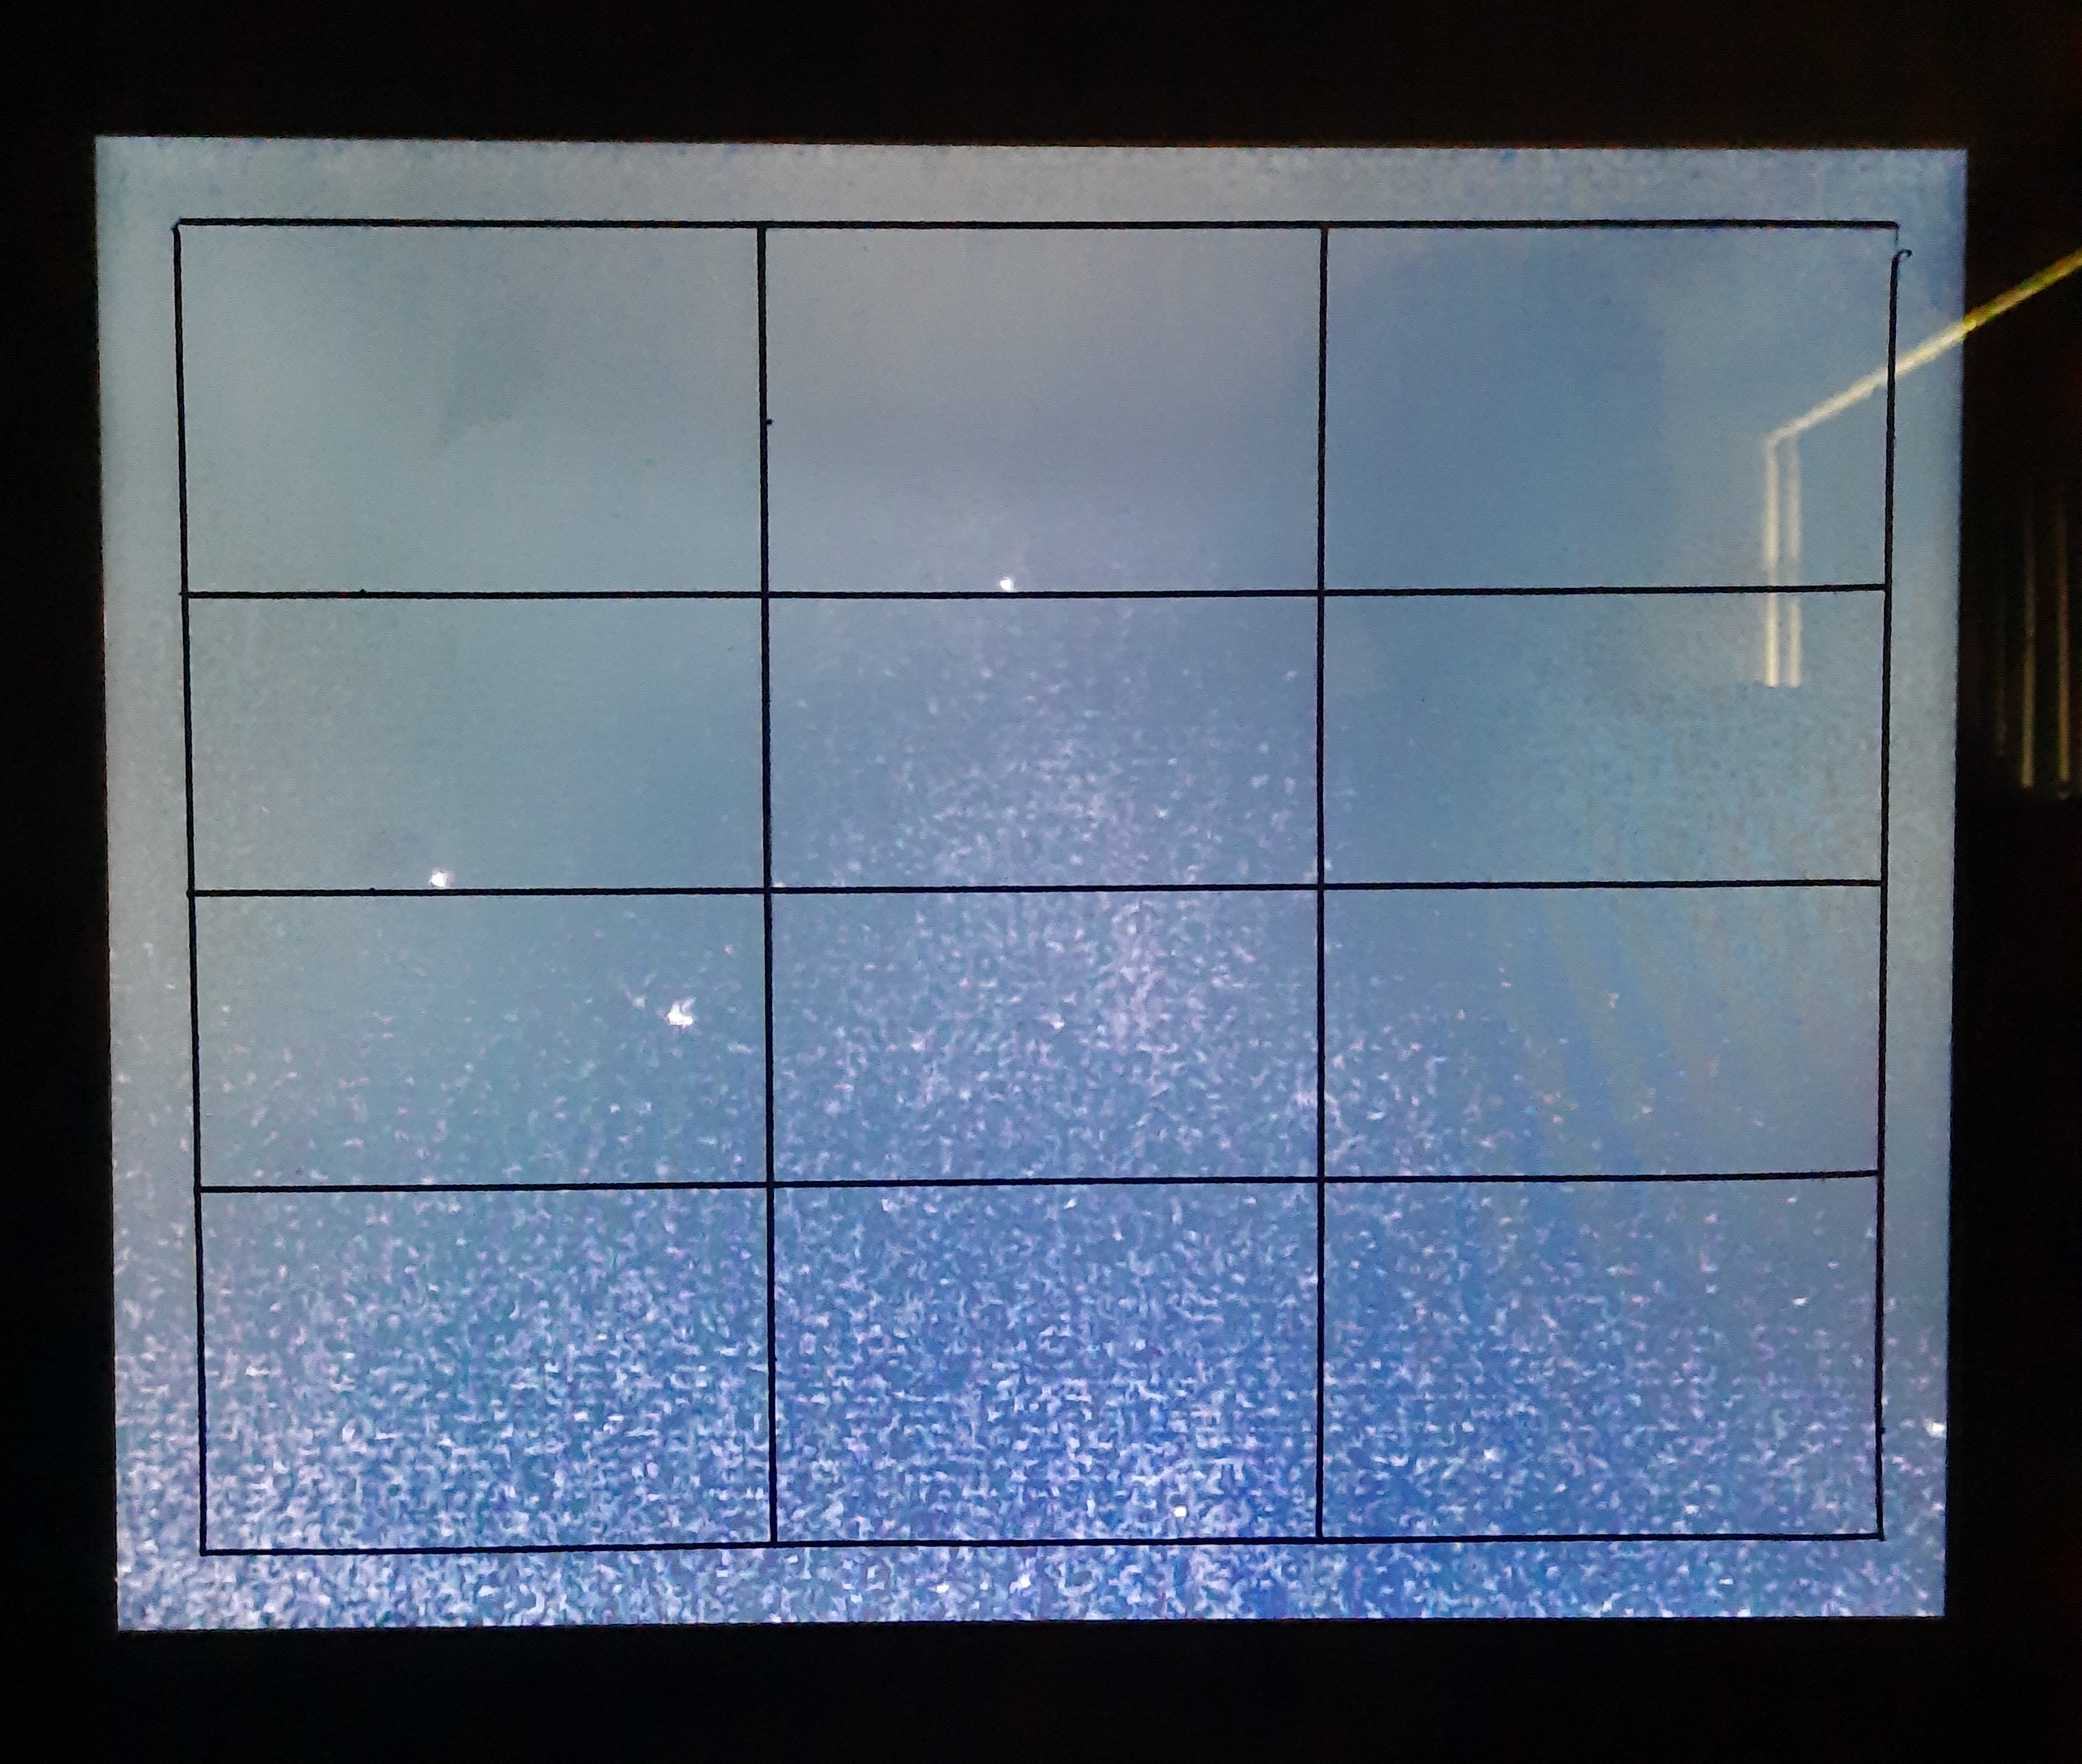
\includegraphics[width=8.3cm,height=6cm]{2} 
	\caption{Constant Deviation Prism}
	\label{1}
\end{figure}

The geometry is as follows:
$$ \angle PQT = \angle BCD=90^{\circ} $$

From Figure (1), we have $\angle$QBC+$\angle$QDC=$180 ^\circ$

$$\angle QBC =90 ^\circ + \theta_r  ;  \angle QDC =90 ^\circ-\theta_i$$

$$\therefore 90 ^\circ+\theta_r+90 ^\circ-\theta_i=180 ^\circ$$

This implies that for $\theta_i=\theta_r$ and emergent ray is $\perp$ to AB, and angle of deviation is $90^\circ$, the ray would be passing through position of minimum deviation. This principle is used in constant deviation spectrometer. 

The bonds of  iodine molecules can vibrate with characteristic energies associated with the quantum state of the molecule. Each electronic state corresponds to particular distribution of certain orbitals. The electronic configuration of lowest energy state is ground state and higher energy states are excited state. In Figure (2), the first three electronic states of molecular iodine is shown.

\begin{figure}[H] %  figure placement: here, top, bottom, or page
	\centering
	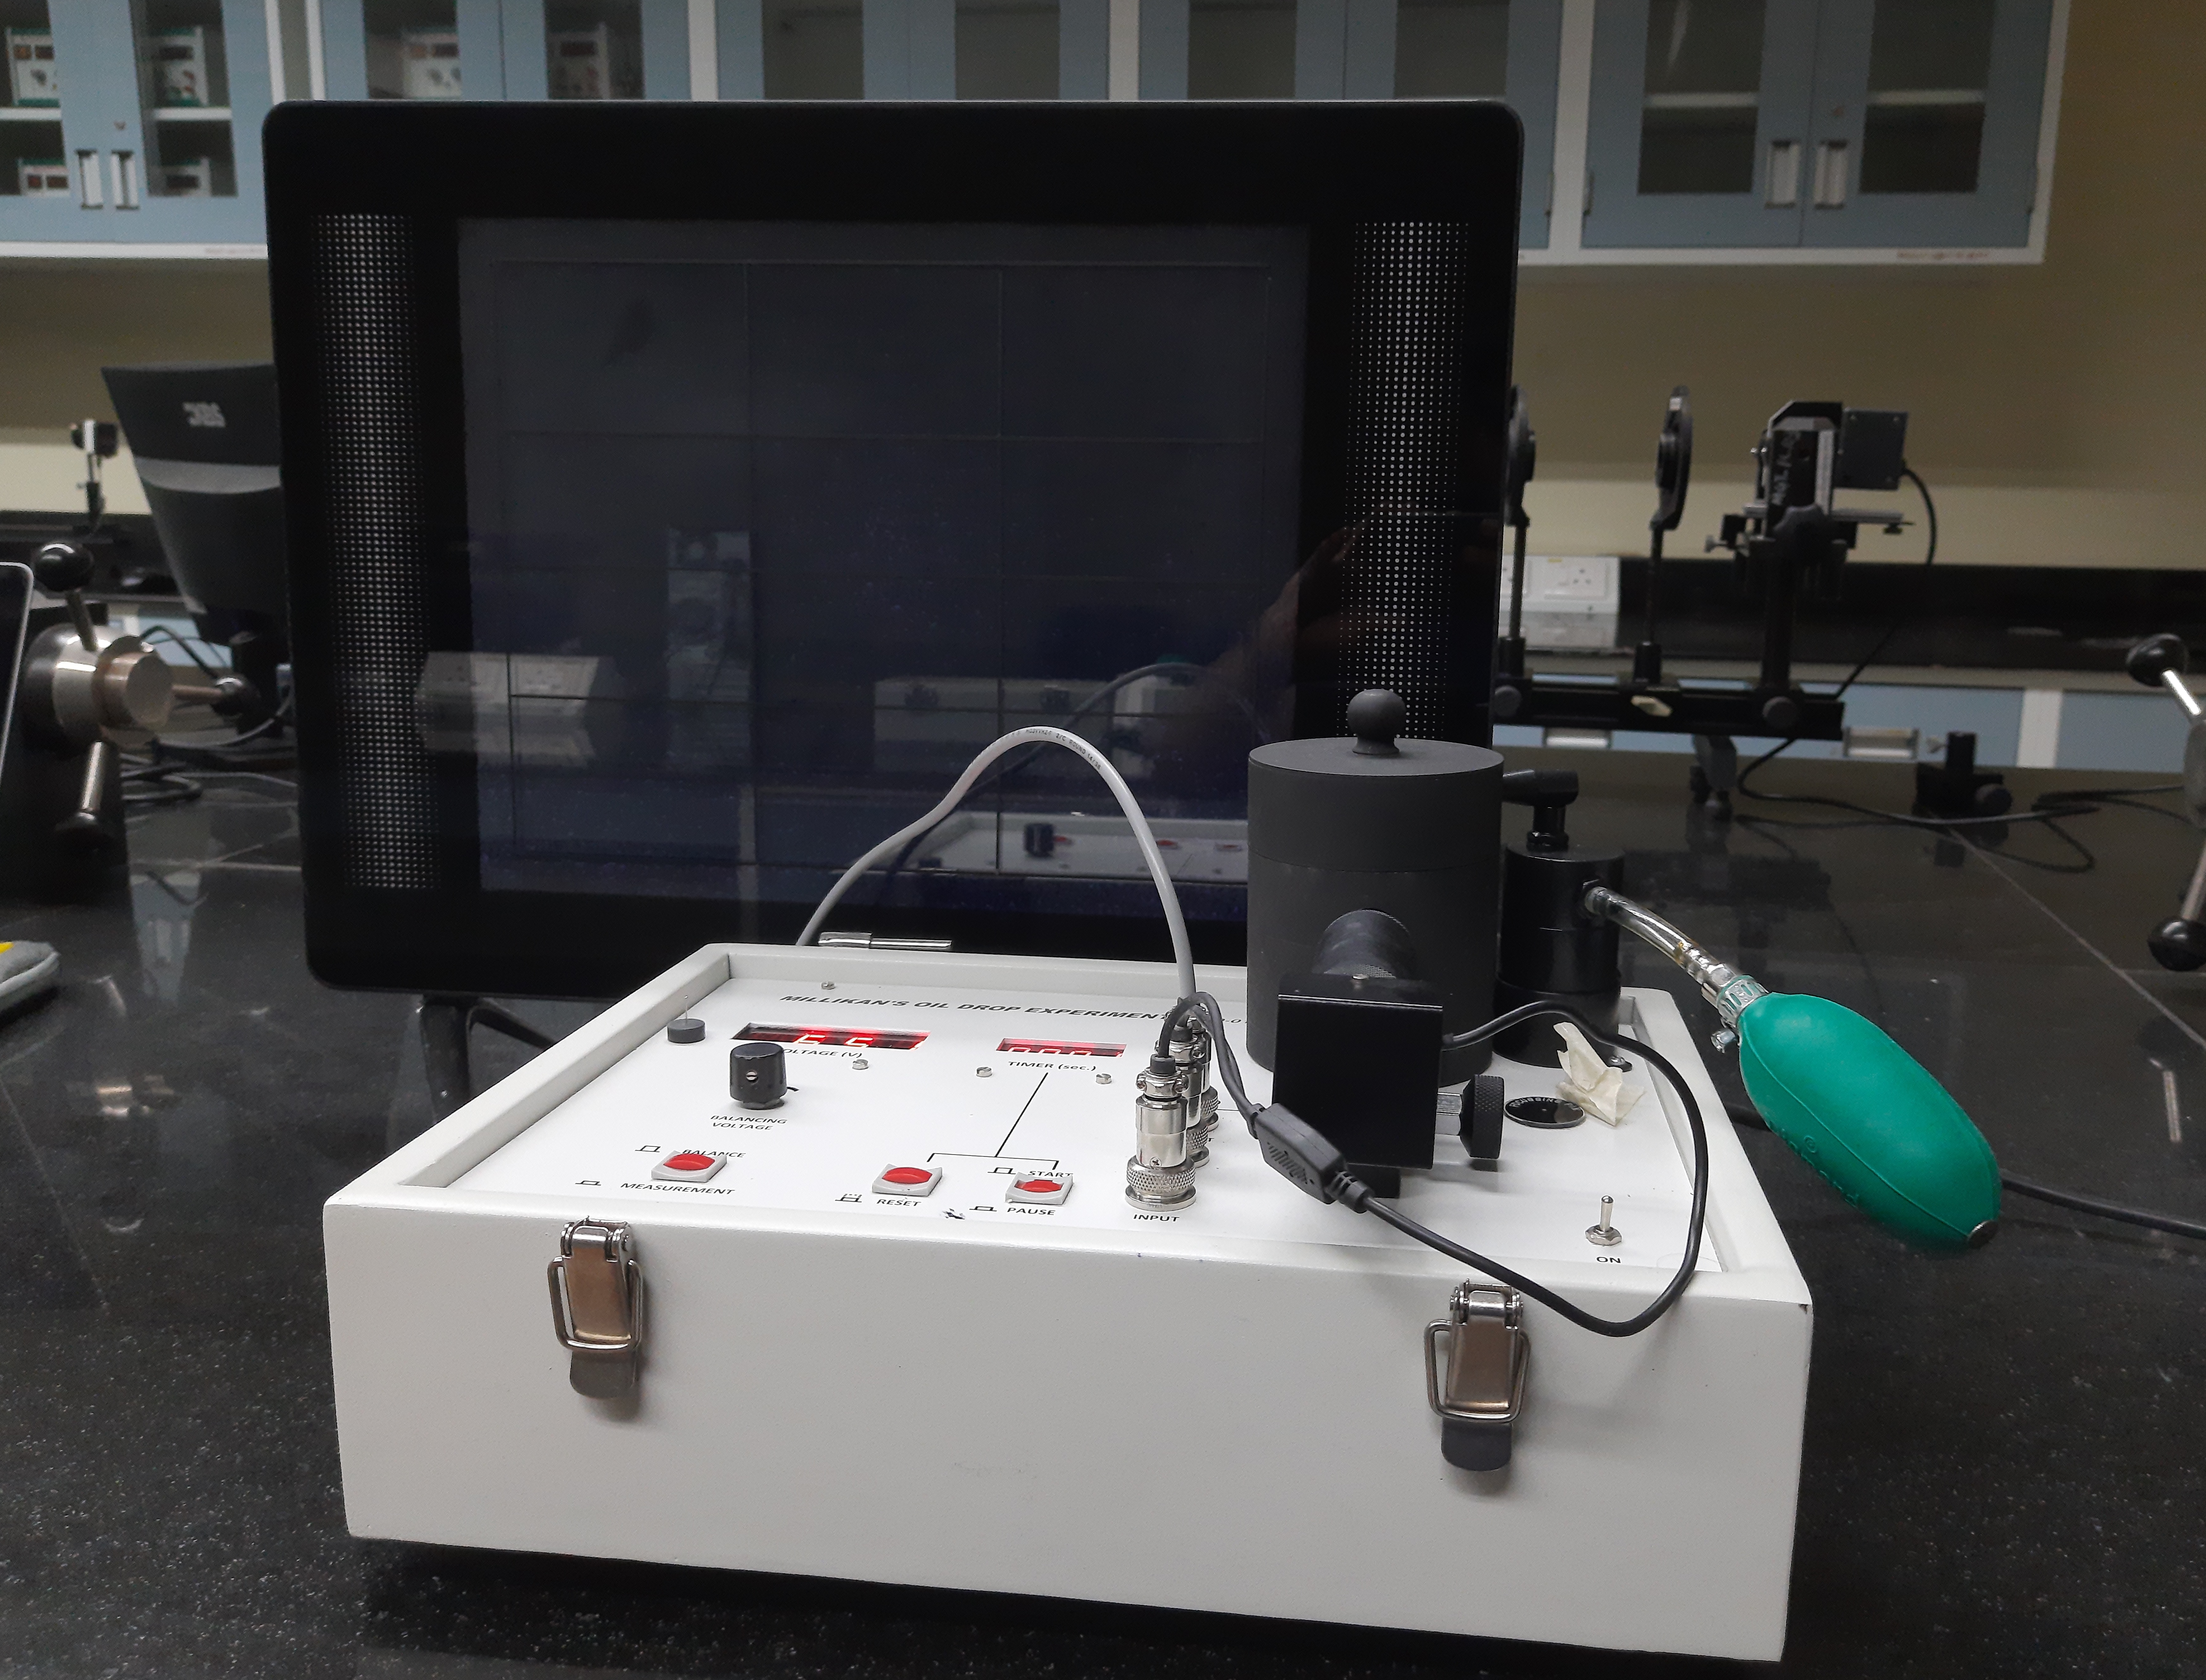
\includegraphics[width=8.3cm,height=6cm]{1} 
	\caption{Potential energy diagram for iodine. X is ground state whereas A and B curves are excited states.}
	\label{2}
\end{figure}

The iodine absorbs light in visible region causing transition between potential curves resulting in a change in the distribution of electrons in the molecule, transitions  between potential curves are also accompanied by changes in vibrational energy. Such transitions are called vibronic.

The potential energy experienced by the electrons in a molecule in any bound state is described by Morse potential:
\begin{equation}
	U(r)=D_e(1-e^{-a(r-r_e)})^2
\end{equation}

where $r$ is the distance between the atoms, $r_e$ is the equilibrium bond distance, $D_e$ is well depth, $a$ is constant for a particular molecule.

\begin{equation}
	a=\bar{\nu_e}\sqrt{\frac{\pi.c.\mu}{\hbar D_e}}
\end{equation}

$ \nu_e $ is the wavenumber corresponding to harmonic vibrational frequency, $\mu$ is the reduced mass of the system. Solving the
Schrodinger equation with Morse potential the vibrational energy states can be obtained as,

\begin{equation}
	E(\nu)=\bar{\nu_e}(\nu+0.5)-\bar{\nu_e}x_e(\nu+0.5)^2
\end{equation}

where $\nu$ is the vibrational quantum number and $x_e$ is the anharmonicity constant.

The iodine under excitation to higher energy states transition is written as ,

$$(X,\nu'')\rightarrow(B,\nu')$$

where X represent ground state, $\nu',\nu''$ represent vibrational quantum numbers in excited ground state, respectively, B is the first excited state.

In ground state $\nu''=0$, But first transition, corresponds to $\nu''=0$ to $\nu'=0$, labelled as 0$\leftarrow$0 absorption line. The next peak
corresponds to the 1←0 transition, so on. According to Franck-Condon principle only those transitions will be more probable where wavefunctions of the two states overlap effectively. For iodine, there is no significant overlap, so transitions are in the range 20 to 50←0, where series of absorption spectrum bands are observed, due to transitions involving excited vibrational levels in ground state and rotation levels.  At the upper edge of the well($\nu'_{max}$) in Figure (2), the vibrational energy spacing decreases to 0, energies forming a continuum rather than being quantized. It is at this limit where bond dissociation occurs. The bond dissociation energy in the excited state ($D_o$) is given by

\begin{equation}
	D_o=E(\nu'=\nu_{max}) -E(\nu'=0)
\end{equation}

One can estimate values of highest and lowest enrgy levels due to absorption. It is observed that vibronic energy levels are coarsel equispaced whereas the difference of the levels decreases towards higher level.To calculate the force constant and energy values, one can use simple harmonic oscillator equations. If $\Delta\bar{\nu}_{e avg}$ is the average value of change in wave number of two consecutive states, then force constant f is 
\begin{equation}
	f=4\pi^2\mu(c\Delta\bar{\nu}_{e avg})^2
\end{equation}

\section{Experiment}
\subsection{Apparatus}
The apparatus consists of constant deviation spectrometer along with voltage source to combust the metallic arcs. The enclosed iodine chamber with incandescent light source is also required.
\subsection{Procedure}

\begin{figure}[H] %  figure placement: here, top, bottom, or page
	\centering
	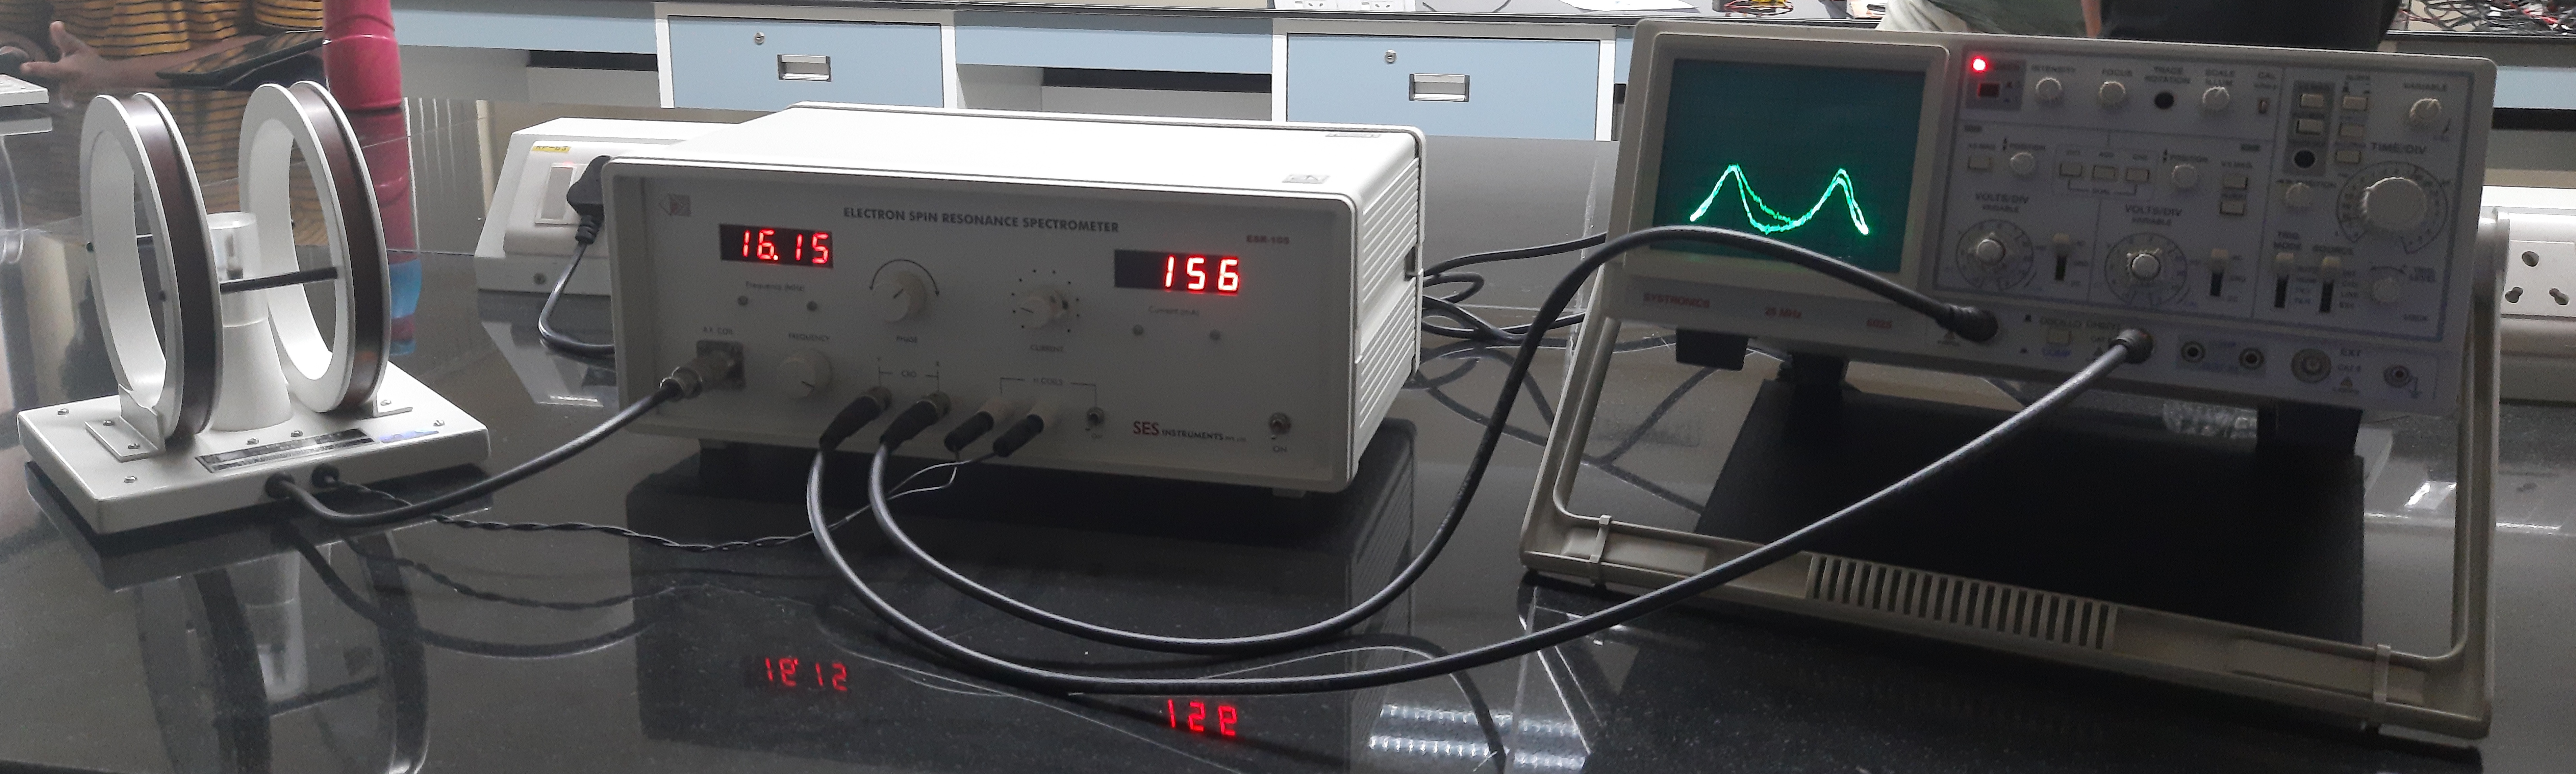
\includegraphics[width=8.3cm,height=6cm]{5} 
	\caption{Schematic diagram for experimental setup}
	\label{5}
\end{figure}

Level the constant deviation spectrometer (CDS) using spirit level. Align the constant deviation prism such that that vertex faces towards objective lens. Use, Hg lamp to calibrate the spectrometer by observing the emission lines. The calibration is done using the rotating drum on CDS where the wavelengths at which emission takes place is known. Note down the readings of the wavelength and plot the actual and observed wavelength to get calibration parameters. Then replace the Hg lamp with metal arc of Cu, Brass. The two pointed metal arc of same material is brought close, connected to DC voltage source, and arc begins to glow. Spectrum is observed and wavelength is noted down. In case of absorption spectrum of I, place the incandescent bulb on the other end of the iodine vapor tube. The light from the tube should pass through the collimator. The absorption spectra is observed and note down the readings of wavelength of the dark bands. From this determine the required parameters like force constant, wave number, bond dissociation energy etc.


\subsection{Precautions}
\begin{enumerate}
	\item {Do not touch the metal arc with bare hands since they are hot and carry very high voltage}
	\item {Bring the pointed arcs close enough to glow it.}
	\item {Maintain the tiny gap between the pointed arcs to avoid excess load on the power supply.}
	\item{Conduct the experiment in the dark room.}
\end{enumerate}


\section{Observation and Analysis}

\begin{figure}[H] %  figure placement: here, top, bottom, or page
	\centering
	\includegraphics[width=5.5cm,height=5.5cm]{7} 
	\caption{Spectral lines of Mercury. There are chromatic aberrations due to which one of the yellow lines appear green.}
	\label{7}
\end{figure}

\begin{figure}[H] %  figure placement: here, top, bottom, or page
	\centering
	\includegraphics[width=8.3cm,height=5.5cm]{3} 
	\caption{Glow of Copper arc during experiment}
	\label{3}
\end{figure}

From the various spectral lines observed, the wavelength of Cu and Brass was corrected and it was found that 8 lines out of 19 observed, were close to the literature value of wavelength, in case of Cu. It is known that Brass is an alloy of Cu and Zn, so both the spectroscopic data of Cu and Zn was taken and was seen that 4 lines of Zn matched with the literature values and rest 7 were from Cu, out of 19 lines observed. The rest lines were not matched as the observed spectral line may be due to impurities present in the metal used. 

\begin{figure}[H] %  figure placement: here, top, bottom, or page
	\centering
	\includegraphics[width=5.5cm,height=5.5cm]{4} 
	\caption{Absorption spectrum of Iodine vapor. Notice dark bands throughout the spectrum.}
	\label{4}
\end{figure}

\begin{figure}[H] %  figure placement: here, top, bottom, or page
	\centering
	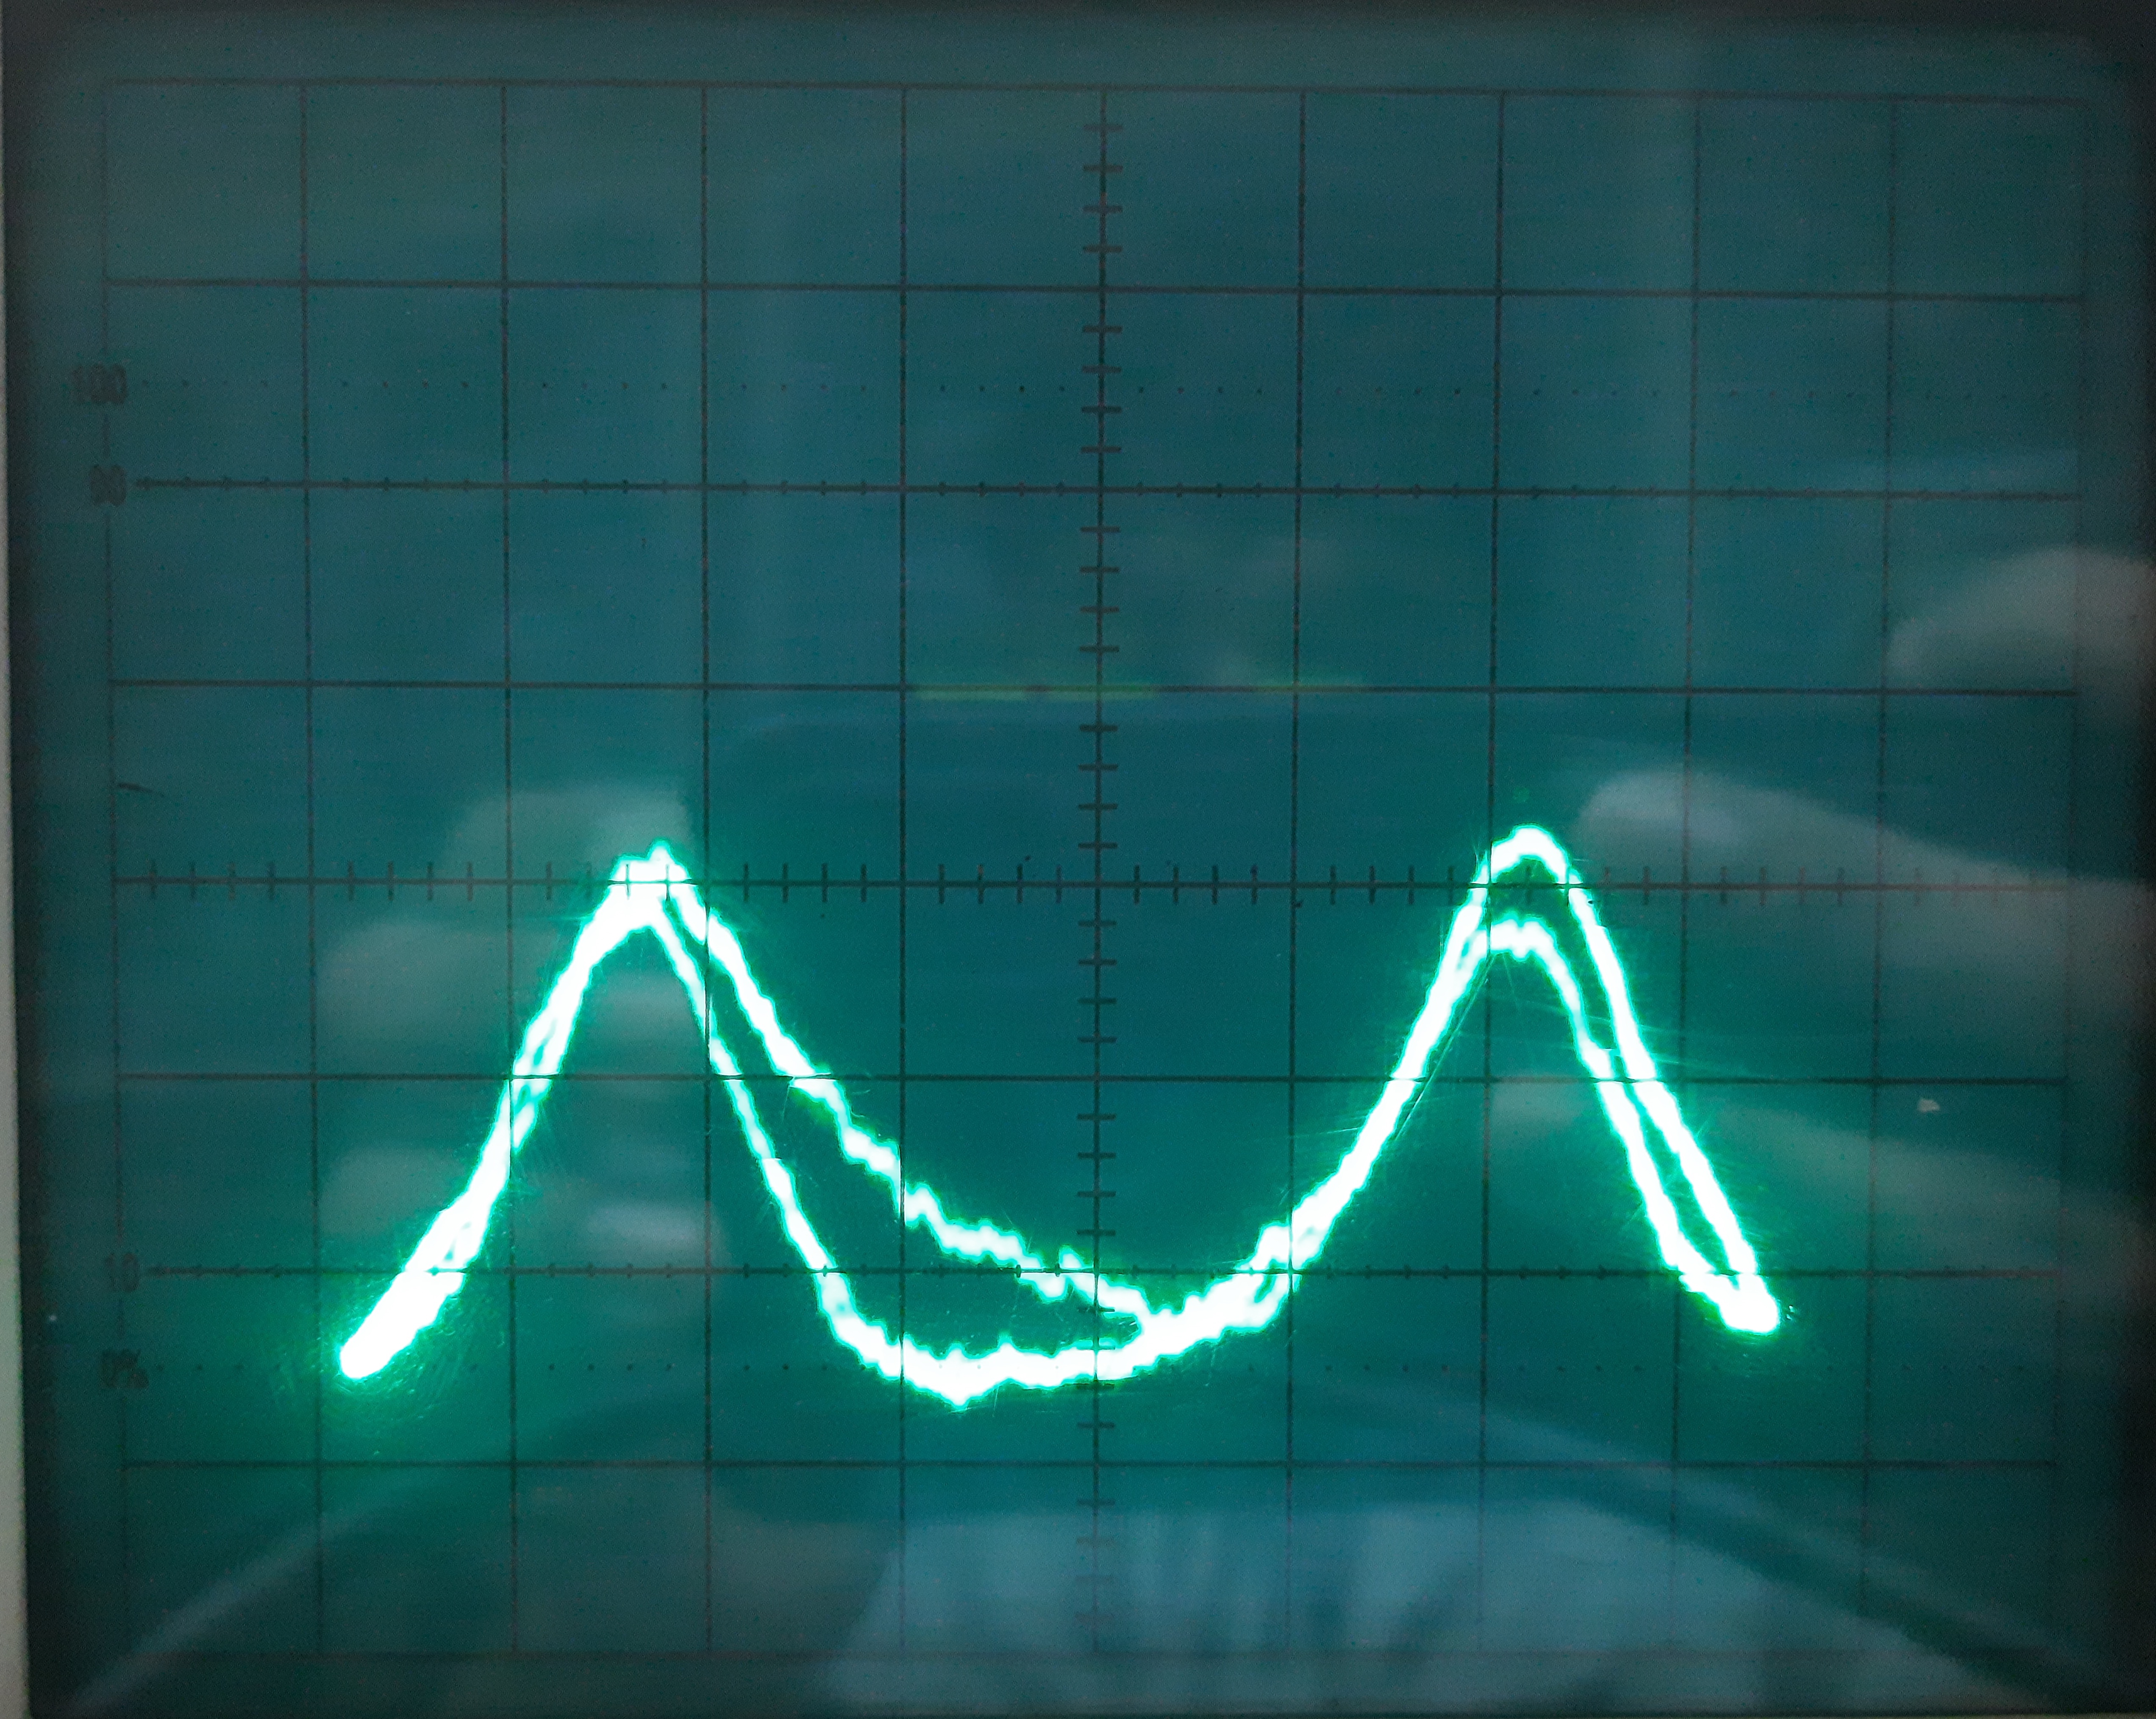
\includegraphics[width=9.3cm,height=6.5cm]{6} 
	\caption{Plot of difference of literature versus observed wavelengths of spectral lines of Mercury to get calibration parameters.}
	\label{6}
\end{figure}

From Figure (7), the calibration equation was found to be 
\begin{equation}
	\lambda_{corr}=(1+m)\lambda_{obs}+c
\end{equation}

where m and c are slope and intercept of plot shown in Figure (7). Therefore, equation (6), turns to 
\begin{equation}
	\lambda_{corr}=(1.00778)\lambda_{obs}-41.5509
\end{equation}

The corrected values of wavelength can be found from equation (7), and compared with the literature values, obtained from various sources from internet. The error in the force constant and other parameters can be found out by standard deviation of the parameter related to it. 

\begin{equation}
	\text{Bond dissociation energy}=h.c(\nu_{max}-nu_{min})
\end{equation}

\begin{equation}
	h.c(17200.94-15531.67)=2.07 meV
\end{equation}

\section{Conclusion and Summary}
 it was seen that not all spectral lines of Cu and brass were matched to their respective literature values due to impurities. Moreover, in case of brass the mixture of Cu and Zn forms hybrid energy level. The absorption spectrum of iodine indicates that its vibrational energy level are equally spaced which implies the potential
 that the electrons in iodine experience can be approximated to be completely harmonic. 
 From the analysis we obtained force constant of iodine in first excited state as $(46.13\pm18.30)$ N/m. The average wave number ($\nu_{e avg})$ was found as $16344.9\pm513.75$ $cm^{-1}$. The bond dissociation energy of iodine is calculated as 2.07 meV. The literature value of bond dissociation energy of iodine is 1.58 eV. 

It is very hard bond dissociation energy to calculate because, not all bands of iodine was absorbed in the visible region as bands after green region gets violet-UV region where it is difficult to observe. Due to this, the error have contributed to the value. With many measurements the value tends to get better. Even the spectrometer with better least count could improve the value as well as reduce the error. Care should be taken while measuring the readings as slight disturbance in the apparatus may given wrong values. 

\section{References}
\begin{enumerate}
	\item{\url{https://www.niser.ac.in/sps/sites/default/files/basic_page/Emission%20Spectra%20of%20Metals%20and%20Absorption%20spectra%20of%20Iodine%20vapour.pdf}}
	\item{\url{https://web.cortland.edu/wheeler/phy150/Laboratory/Laboratory1.pdf}}
	\item{\url{http://hyperphysics.phy-astr.gsu.edu/hbase/quantum/atspect2.html#c2}}
	\item{\url{https://physicsopenlab.org/2022/07/10/iodine-vapor-absorption/}} 
	\item{\url{https://instructional-resources.physics.uiowa.edu/demos/7b1020-spectral-linesspectroscopy-mercury-emission-lines-0}}
	\item{\url{http://people.uncw.edu/olszewski/phy102lab/laboratory/mercury.pdf}}
	\item{\url{https://www.nist.gov/pml/handbook-basic-atomic-spectroscopic-data}}
	\item{\url{https://www.colby.edu/chemistry/PChem/Hartree.html}}
	\item{\url{https://labs.chem.ucsb.edu/zakarian/armen/11---bonddissociationenergy.pdf}}
\end{enumerate}

\end{document}